
\chapter{ಮಾಯಾ ಆಕೃತಿಗಳು (Magic Figures) ಮತ್ತು ಮಾಯಾ ನಕ್ಷತ್ರಗಳು}

ನಮಗೆ ಗೊತ್ತೇ ಇದೆ. ಮಾಯಾಚೌಕವೆಂದರೆ ಒಂದು ಚೌಕ. ಚಚ್ಚೌಕ (Square). ಉದ್ದ, ಅಗಲ\-ಗಳನ್ನು ಸಮಾನ ಸಂಖ್ಯೆಯ ಭಾಗಗಳಾಗಿ ಮಾಡಿ ರಚಿಸಿರುವ ಹಂದರದಲ್ಲಿ ಸಂಖ್ಯೆ\-ಗಳನ್ನು ತುಂಬಿಸಿರುವುದು. ಅಡ್ಡಸಾಲು, ಕಂಭಸಾಲು ಮತ್ತು ಕರ್ಣಗಳಲ್ಲಿನ ಸಂಖ್ಯೆಗಳ ಮೊತ್ತ ಒಂದು ಚೌಕಕ್ಕೆ ನಿರ್ದಿಷ್ಟ. ಅನೇಕ ಗಣಿತಜ್ಞರು ಈ ದಿಶೆಯಲ್ಲಿ ಕೆಲಸಮಾಡಿ ಸಾವಿರಾರು ವಿನೂತನ, ವಿಶಿಷ್ಟ ಮಾಯಾಚೌಕಗಳನ್ನು ಪಡೆದಿರುವುದು ನಮಗೇ ವೇದ್ಯ.

ಕೆಲವು ಗಣಿತಜ್ಞರು ಹಾಗೂ ಮಾಯಾಚೌಕಾಸಕ್ತರು ಈ ಚೌಕಟ್ಟನ್ನು ದಾಟಿ ಬೇರೆ \hbox{ಜ್ಯಾಮಿತೀಯ} ಆಕೃತಿಗಳ ಬಾಹುಗಳ ಮೇಲೆ ಸಂಖ್ಯೆ ಹಾಕಿ, ಮೊತ್ತ ಒಂದು ನಿರ್ದಿಷ್ಟ ಸಂಖ್ಯೆ ಯಾಗುವುದನ್ನು ಪ್ರಯತ್ನಿಸಿದ್ದಾರೆ. ಅದರಲ್ಲಿ ಯಶಸ್ಸನ್ನೂ ಗಳಿಸಿದ್ದಾರೆ. ಇವುಗಳಿಗೆ \break \textbf{‘‘ಮಾಯಾ ಆಕೃತಿ’’} ಗಳೆಂದು ಹೆಸರಿಸಲಾಗಿದೆ. ಅಂತಹ ಕೆಲವನ್ನು ಗಮನಿಸೋಣ.

\section*{* ಮಾಯಾ ತ್ರಿಭುಜಗಳು :}

ಸರಳ ರೇಖೆಗಳಿಂದಾಗಬಹುದಾದ ಆಕೃತಿಗಳಲ್ಲಿ ತ್ರಿಭುಜವೇ ಅತಿ ಸರಳ. ಕನಿಷ್ಠ ಸಂಖ್ಯೆಯ ಸರಳ ರೇಖೆಗಳಿಂದ ರಚಿಸಬಹುದಾದುದು. ತ್ರಿಭುಜದ ಶೃಂಗ ಮತ್ತು ಬಾಹುಗಳ ಮೇಲೆ ಸಂಖ್ಯೆ\-ಗಳನ್ನು ಬರೆದು, ಒಂದೊಂದು ಬಾಹುವಿನ ಮೇಲೆ ಬರುವ ಸಂಖ್ಯೆಗಳ ಮೊತ್ತ ಒಂದು \hbox{ತ್ರಿಭುಜಕ್ಕೆ} ಸ್ಥಿರಾಂಕವಾದರೆ ಅದನ್ನು ಮಾಯಾತ್ರಿಭುಜವೆನ್ನಬಹುದು. ಇವುಗಳನ್ನು ರಚಿಸು\-ವುದು ಸುಲಭವೇ. ಇವುಗಳಲ್ಲಿ ಅಂತಹ ಕುತೂಹಲಕಾರಿ ಅಂಶಗಳೇನೂ ಇಲ್ಲ. ಕೆಲವು \hbox{ಮಾಯಾ} ತ್ರಿಭುಜಗಳನ್ನು ನೋಡಿ.
\begin{figure}[H]
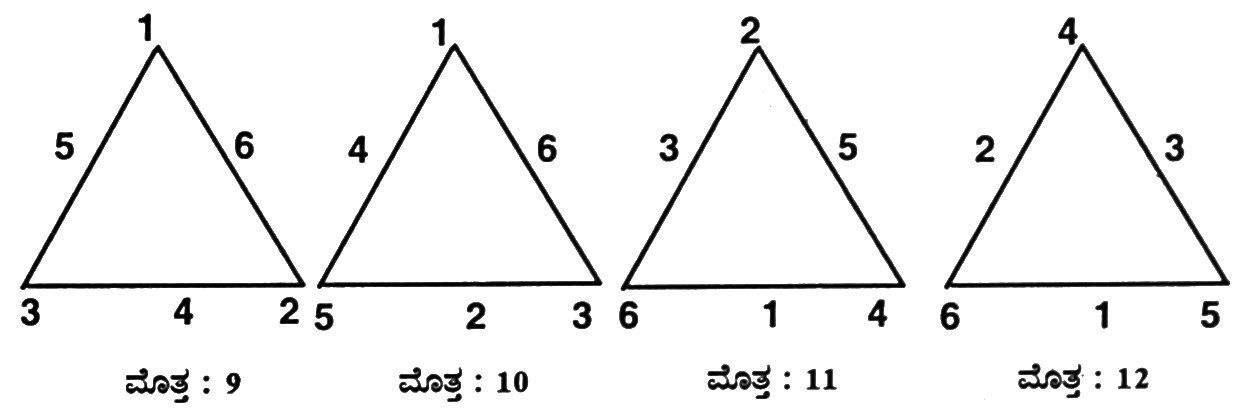
\includegraphics[scale=.8]{src/figures/chap8/fig8-1.jpg}
\end{figure}

ತ್ರಿಭುಜಗಳು ಸಮಬಾಹು ತ್ರಿಭುಜಗಳೇ ಆಗಬೇಕೆಂದಿಲ್ಲ. ಉದಾಹರಣೆಯಲ್ಲಿ 1 ರಿಂದ 6ರವರೆಗಿನ ಸಂಖ್ಯೆಗಳನ್ನು ಮಾತ್ರ ಬಳಸಿದೆ. ಮೊತ್ತ ಬೇರೆ ಬೇರೆಯಾಗಿರುವುದನ್ನು ಗಮನಿಸಿ.

\section*{* ಮಾಯಾ ಪಂಚಭುಜ :}

4 ಭುಜಗಳ ಆಕೃತಿಗಳನ್ನು ಪರಿಗಣಿಸಿಲ್ಲ. ಎಲ್ಲ ಮಾಯಾಚೌಕಗಳು 4 ಭುಜಗಳ ಆಕೃತಿಗಳೇ. ಮಾಯಾಪಂಚಭುಜಾಕೃತಿಗೆ ಒಂದು ಮಾದರಿ.
\begin{figure}[H]
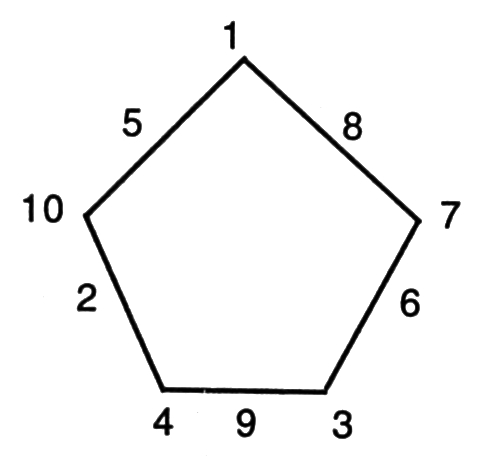
\includegraphics[scale=.6]{src/figures/chap8/fig8-2.jpg}
\end{figure}
\begin{itemize}
	\item 1 ರಿಂದ 10ರವರೆಗೆ ಕ್ರಮಾಗತ ಸಂಖ್ಯೆಗಳು.
	\item ಯಾವುದೇ ಬಾಹುವಿನ ಮೇಲೆ ಇರುವ ಸಂಖ್ಯೆಗಳ ಮೊತ್ತ 16.
\end{itemize}

ಇಂತಹ ಆಕೃತಿಗಳಲ್ಲಿ ಹೆಚ್ಚು ವಿಸ್ಮಯ ಕಂಡುಬರುವುದಿಲ್ಲ. ಆಸಕ್ತರು ಸ್ವಲ್ಪ ತಾಳ್ಮೆ ಮತ್ತು ಪರಿಶ್ರಮ ಹಾಕಿದರೆ ರಚಿಸಲು ಸಾಧ್ಯ. ಇನ್ನೂ ಹೆಚ್ಚಿನ ಬಾಹುಗಳಿರುವ ಆಕೃತಿಗಳನ್ನು ರಚಿಸಬಹುದು.

ಇವುಗಳಿಗಿಂತ ಮಾಯಾನಕ್ಷತ್ರಗಳು ಭಿನ್ನ. ಅವು ಸರಳ ರೇಖೆಗಳಿಂದಾದ ನಕ್ಷತ್ರ ಆಕೃತಿಯವು. 5 ಮತ್ತು ಮೇಲ್ಪಟ್ಟ ಸಂಖ್ಯೆಗಳಷ್ಟು ಶೃಂಗಗಳನ್ನು ಹೊಂದಿರುವ ನಕ್ಷತ್ರಗಳನ್ನು ರಚಿಸಲಾಗಿದೆ. ಇವುಗಳಲ್ಲಿ ಸರಳ ರೇಖೆಗಳ ಮೇಲೆ ಬರುವ ಶೃಂಗ ಮತ್ತು ಛೇದನ ಬಿಂದುಗಳಲ್ಲಿ ಸಂಖ್ಯೆಗಳನ್ನು ಬರೆಯಲಾಗುತ್ತದೆ. ಯಾವುದೇ ಸರಳ ರೇಖೆಯ ಮೇಲೆ ಬರುವ ಸಂಖ್ಯೆಗಳ ಮೊತ್ತ ನಿರ್ದಿಷ್ಟ.

ಕೆಲವು ಮಾಯಾನಕ್ಷತ್ರಗಳನ್ನು ಪರಿಶೀಲಿಸೋಣ.

\section*{* 5. ಶೃಂಗಗಳ ನಕ್ಷತ್ರ:} 

ಯಾವುದೇಬಾಹುವಿನಮೇಲಿನ ಸಂಖ್ಯೆಗಳ ಮೊತ್ತ 24.
\begin{figure}[H]
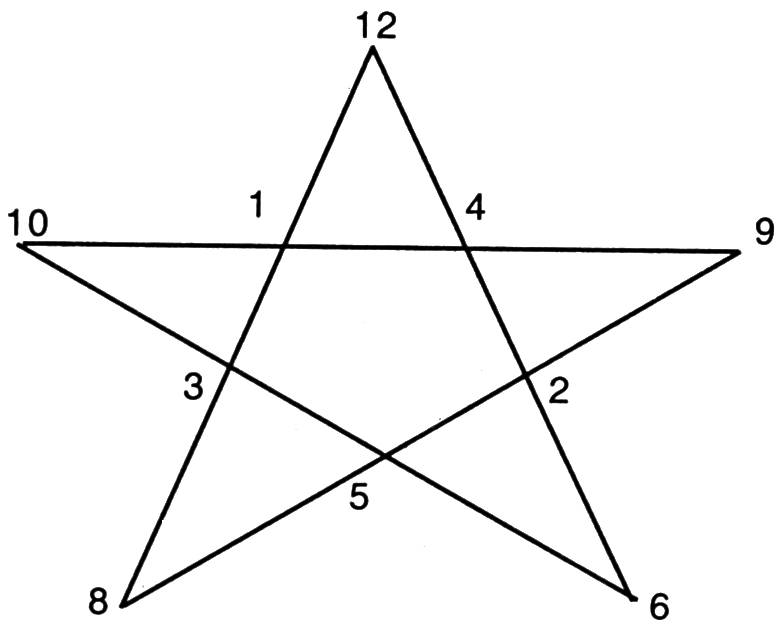
\includegraphics[scale=.6]{src/figures/chap8/fig8-3.jpg}
\end{figure}

\section*{* 6. ಶೃಂಗಗಳ ನಕ್ಷತ್ರ:} 

\begin{figure}[H]
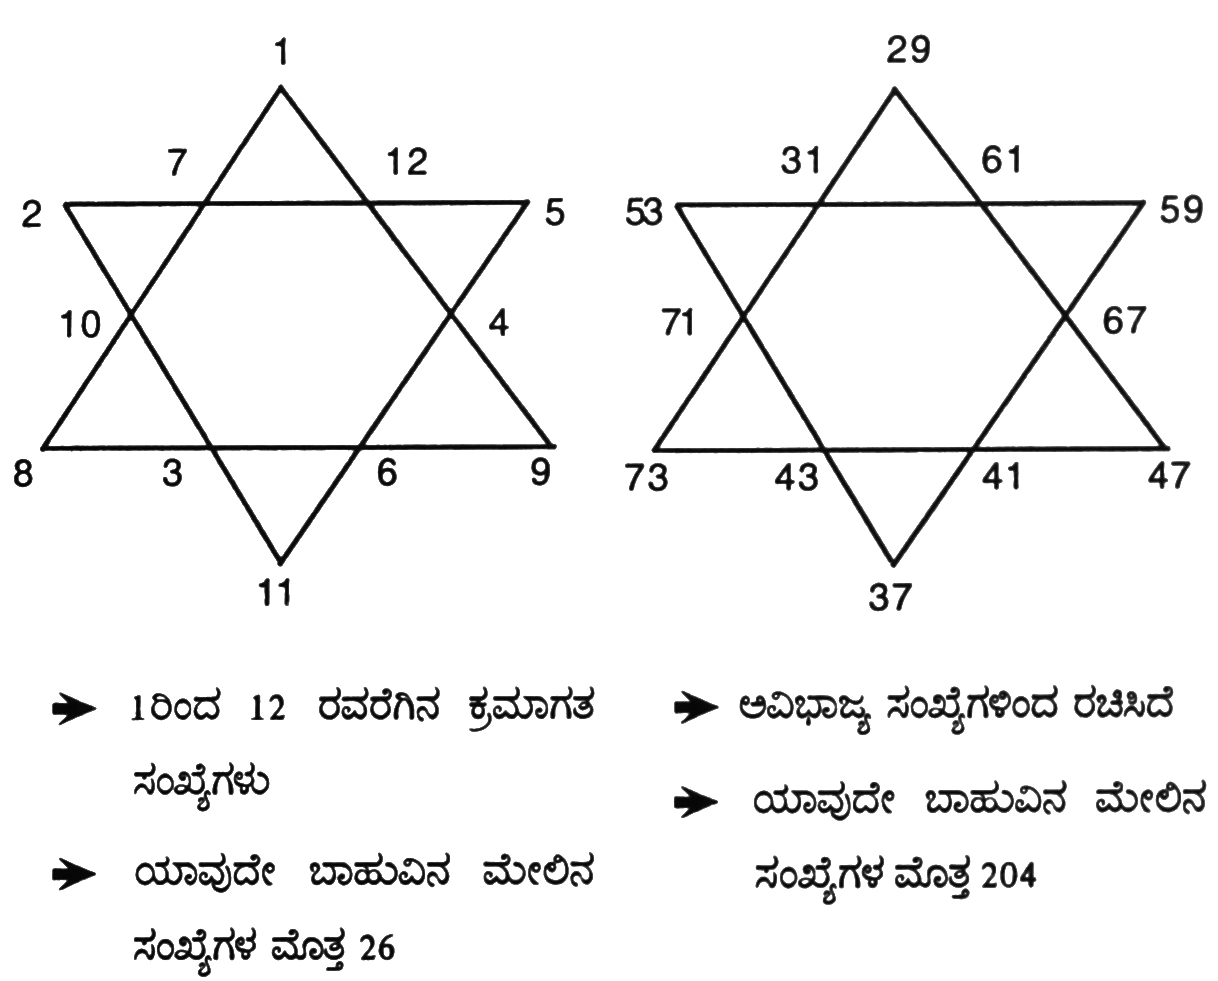
\includegraphics[scale=.9]{src/figures/chap8/fig8-4.jpg}
\end{figure}

\section*{* 7. ಶೃಂಗಗಳ ನಕ್ಷತ್ರ:} 

1ರಿಂದ 14ರವರೆಗೆ ಕ್ರಮಾಗತ ಸಂಖ್ಯೆಗಳು. ಮೊತ್ತ : 30
\begin{figure}[H]
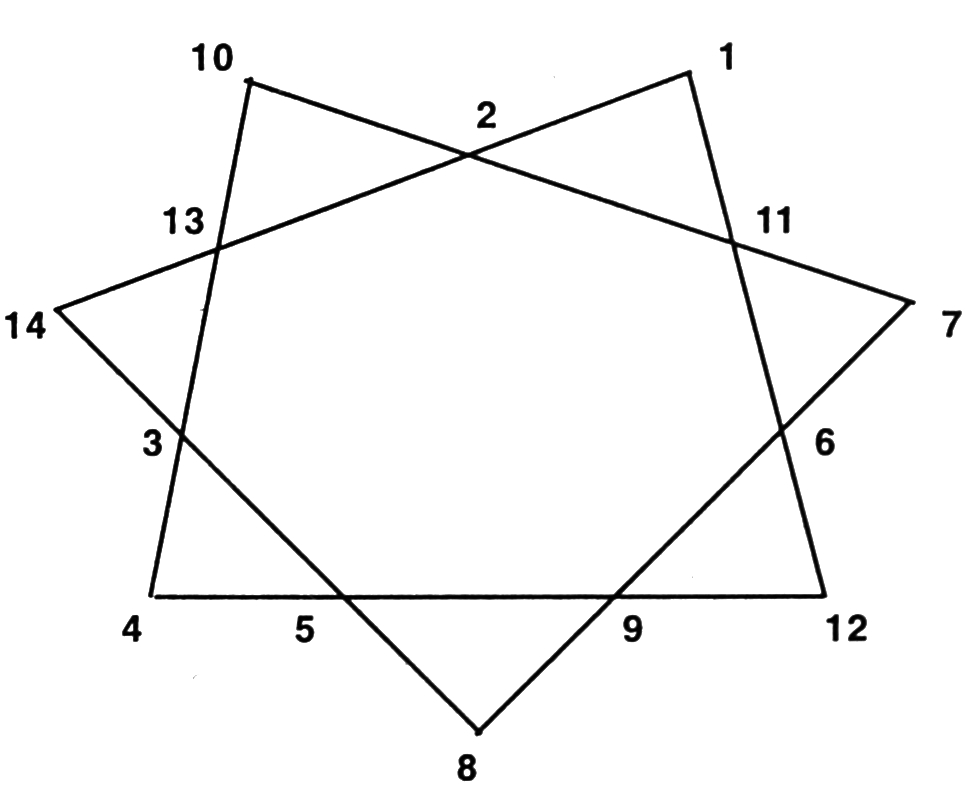
\includegraphics[scale=.8]{src/figures/chap8/fig8-5.jpg}
\end{figure}

\section*{* 8 ಶೃಂಗಗಳ ನಕ್ಷತ್ರ :}

\begin{figure}[H]
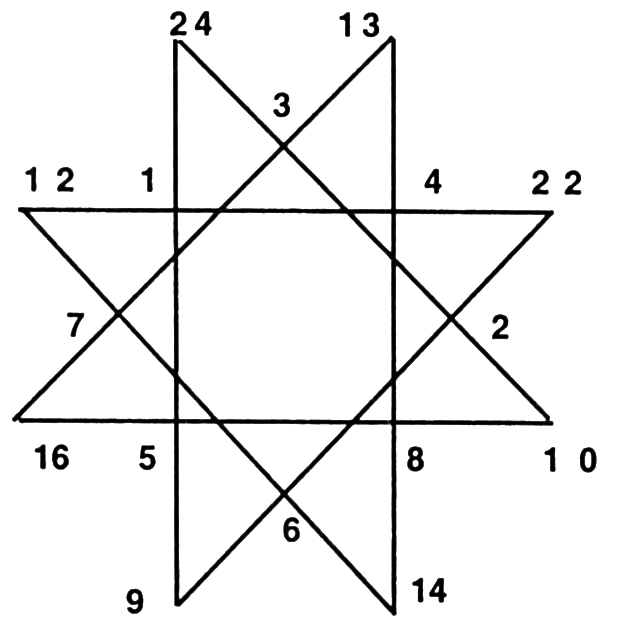
\includegraphics[scale=.9]{src/figures/chap8/fig8-6.jpg}
\end{figure}

$\bullet$ ಸಂಖ್ಯೆಗಳು ಕ್ರಮಾಗತವಾಗಿಲ್ಲ. ಮೊತ್ತ : 39
\begin{figure}[H]
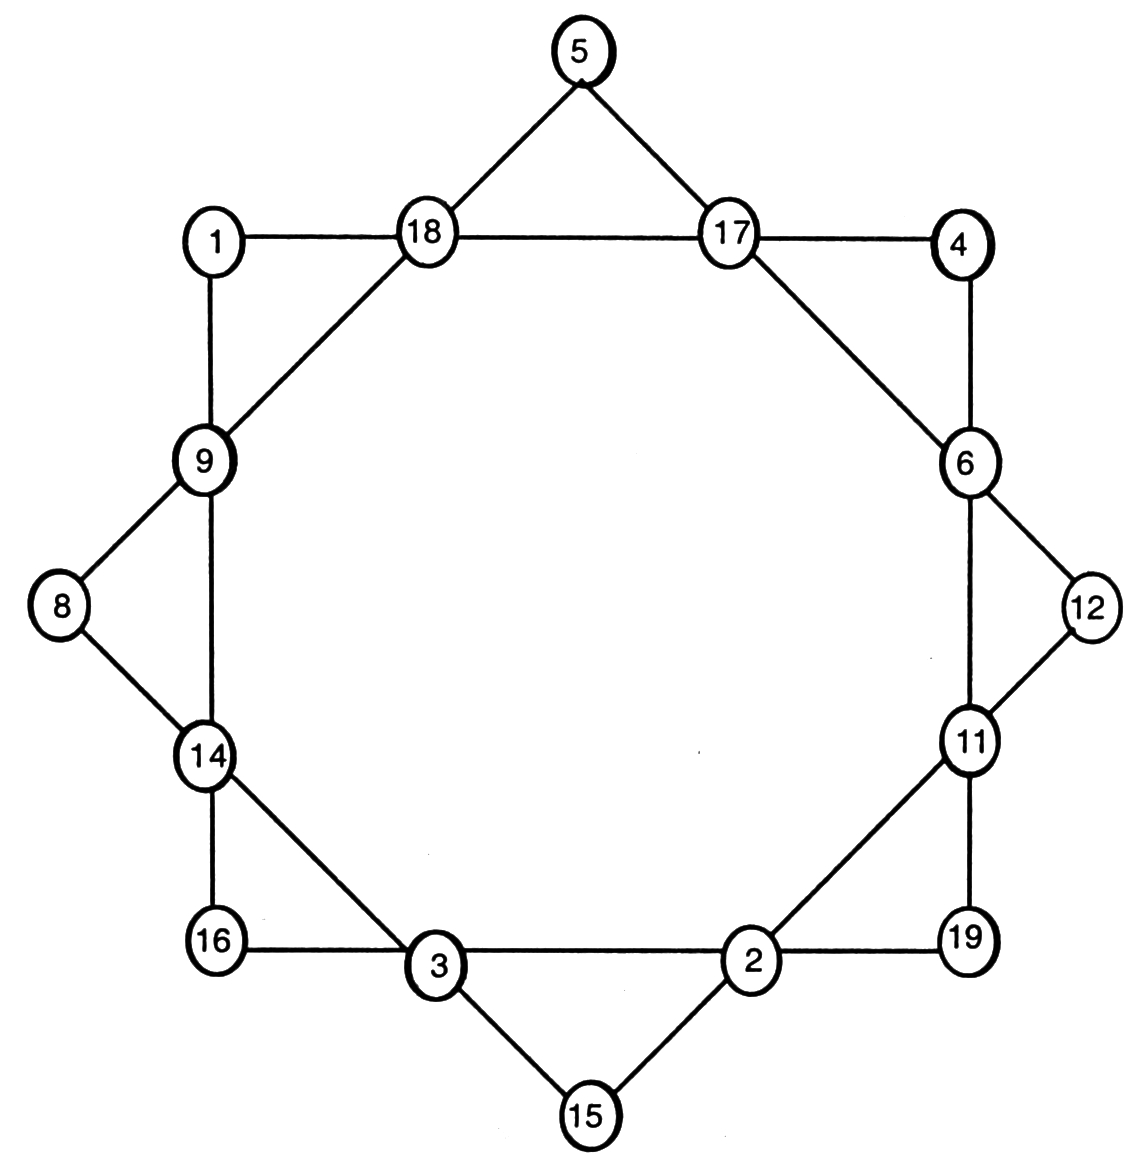
\includegraphics[scale=.8]{src/figures/chap8/fig8-7.jpg}
\end{figure}

$\bullet$ ಸಂಖ್ಯೆಗಳು ಕ್ರಮಾಗತವಾಗಿಲ್ಲ. ಮೊತ್ತ : 40
\section*{IX- 2. ಮಾಯಾ ಜೇನುಗೂಡು (Magic Honey Comb)}

\begin{figure}[H]
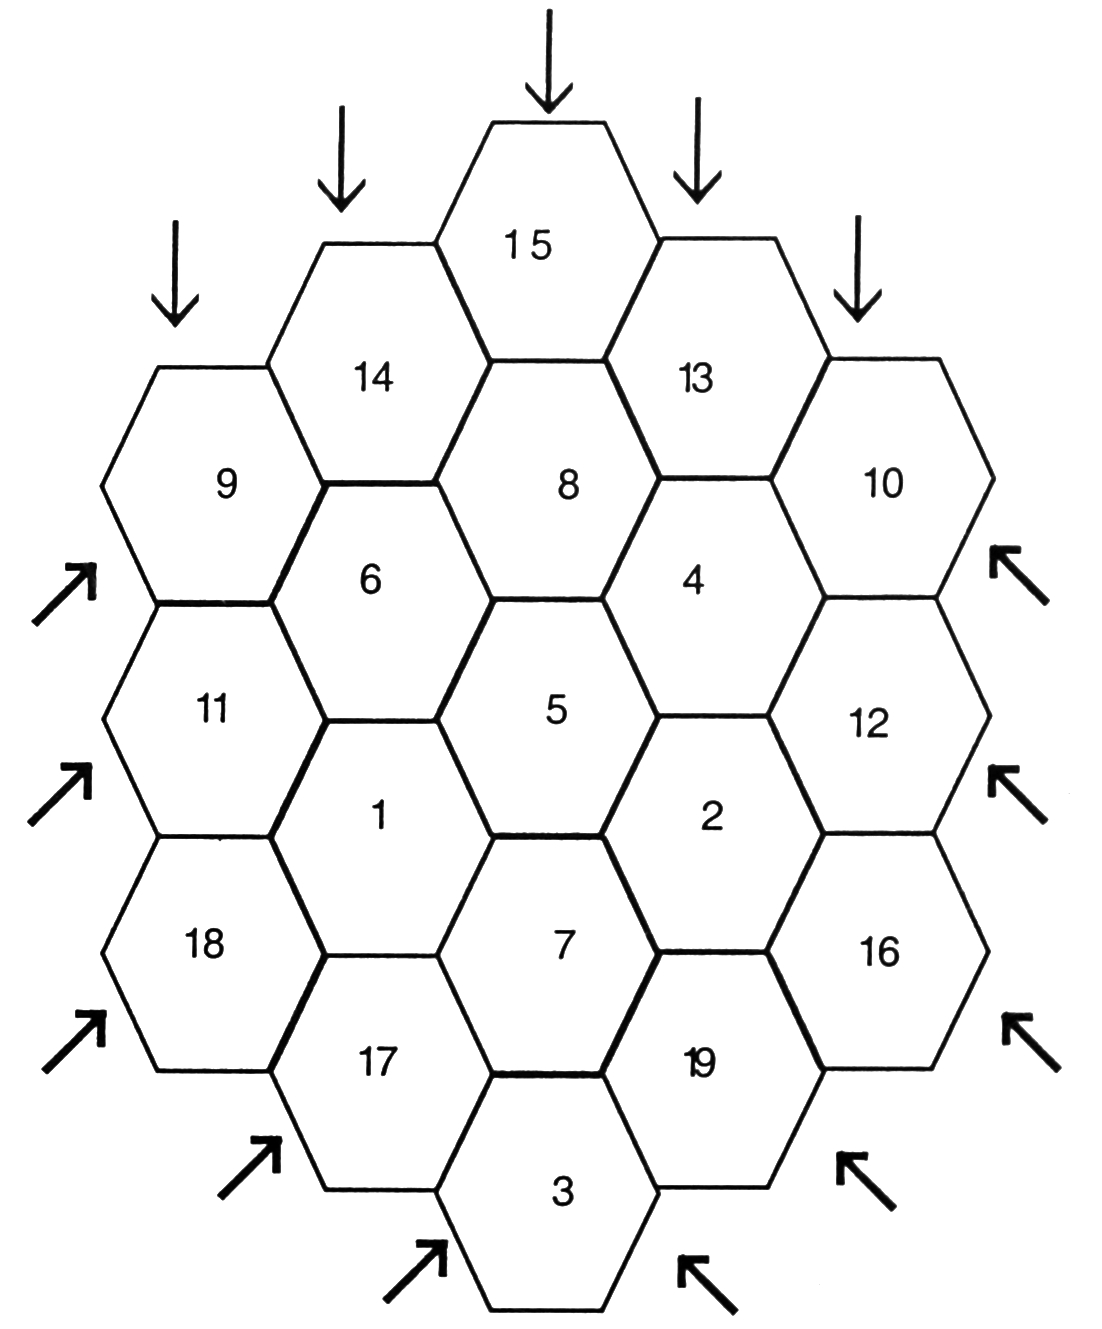
\includegraphics{src/figures/chap8/fig8-8.jpg}
\end{figure}
\begin{itemize}
	\item 1ರಿಂದ 19ರವರೆಗಿನ ಕ್ರಮಾಗತ ಸಂಖ್ಯೆಗಳನ್ನು ಬಳಸಲಾಗಿದೆ.\smallskip
	\item ಎಲ್ಲ ಮನೆಗಳೂ ಷಡ್ಭುಜಾಕೃತಿಗಳು.\smallskip
	\item ಬಾಣದ ಗುರುತಿನ ನೇರದಲ್ಲಿ ಬರುವ ಷಡ್ಭುಜಗಳೊಳಗಿನ ಸಂಖ್ಯೆಗಳ ಮೊತ್ತ $\boxed{38}$
\end{itemize}

\section*{* ಮಾಯಾ ಷಡ್ಭುಜ :}

\begin{figure}[H]
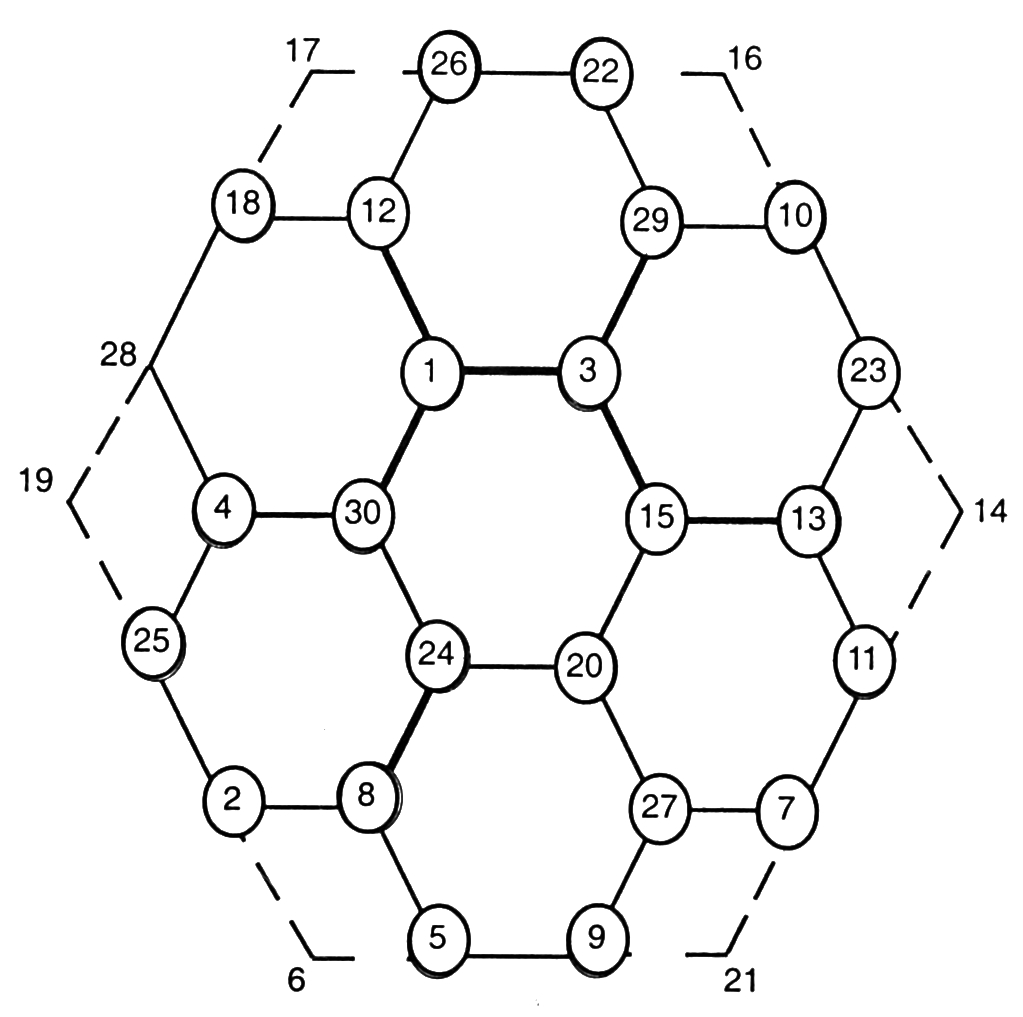
\includegraphics[scale=1.1]{src/figures/chap8/fig8-9.jpg}
\end{figure}
\begin{itemize}
	\item 1ರಿಂದ 30 ರವರೆಗಿನ ಕ್ರಮಾಗತ ಸಂಖ್ಯೆಗಳನ್ನು ಬಳಸಲಾಗಿದೆ.\smallskip
	\item ಒಂದು ಕೇಂದ್ರ ಷಡ್ಭುಜಾಕೃತಿಗೆ ಲಗತ್ತಾದಂತೆ 6 ಷಡ್ಭುಜಗಳಿವೆ.\smallskip
	\item ಯಾವುದೇ ಷಡ್ಭುಜದ ಶೃಂಗ ಸಂಖ್ಯೆಗಳ ಮೊತ್ತ 93\smallskip
	\item ಗೀಟು ರೇಖೆಗಳನ್ನೊಳಗೊಂಡ ಒಂದು ದೊಡ್ಡ ಷಡ್ಭುಜವಿದೆ. ಇದರ ಶೃಂಗ ಸಂಖ್ಯೆ\-ಗಳು 17,16,14,21,6,19. ಇವುಗಳ ಮೊತ್ತವೂ 93.
\end{itemize}
\begin{center}
*****
\end{center}

\section*{IX. 3. ಪೈಥಾಗೊರಾಸ್ ತ್ರಿವಳಿಗಳಿಂದಾದ ಮಾಯಾಚೌಕ :}

ಪೈಥಾಗೊರಾಸ್ ಪ್ರಮೇಯ ಹೀಗೆ ಹೇಳುತ್ತದೆ. ಒಂದು ಲಂಬ ಕೋನ ತ್ರಿಭುಜದಲ್ಲಿ ಕರ್ಣರೇಖೆಯ ಮೇಲಿನ ವರ್ಗದ ವಿಸ್ತೀರ್ಣವು ಉಳಿದೆರಡು ಬಾಹುಗಳ ಮೇಲೆ ರಚಿಸಿದ ವರ್ಗಗಳ ವಿಸ್ತೀರ್ಣದ ಮೊತ್ತಕ್ಕೆ ಸಮ. $ABC$ ತ್ರಿಭುಜವು ಅಯಲ್ಲಿ ಲಂಬಕೋನ ಹೊಂದಿರಲಿ. $BC$ ಕರ್ಣ, ಆಗ $BC^2 = AB^2 +AC^2$. 

\medskip
ಒಂದು ಲಂಬಕೋನ, ತ್ರಿಭುಜ $ABC$ಯಲ್ಲಿ $BC$ ಕರ್ಣವಾಗಿರಲಿ. $BC$, $AB$ ಮತ್ತು $AC$ಗಳ ಮೇಲೆ ಚೌಕಗಳನ್ನು ರಚಿಸಿ. ಮೂರು ಚೌಕಗಳನ್ನೂ $3 \times 3$ ಇರುವಂತೆ \break ವಿಭಾಗಿಸಿ. ಚಿತ್ರದಲ್ಲಿರುವಂತೆ ಸಂಖ್ಯೆಗಳನ್ನು 3 ಚೌಕಗಳ ಮನೆಗಳಲ್ಲೂ ತುಂಬಿಸಿ.
\begin{figure}[H]
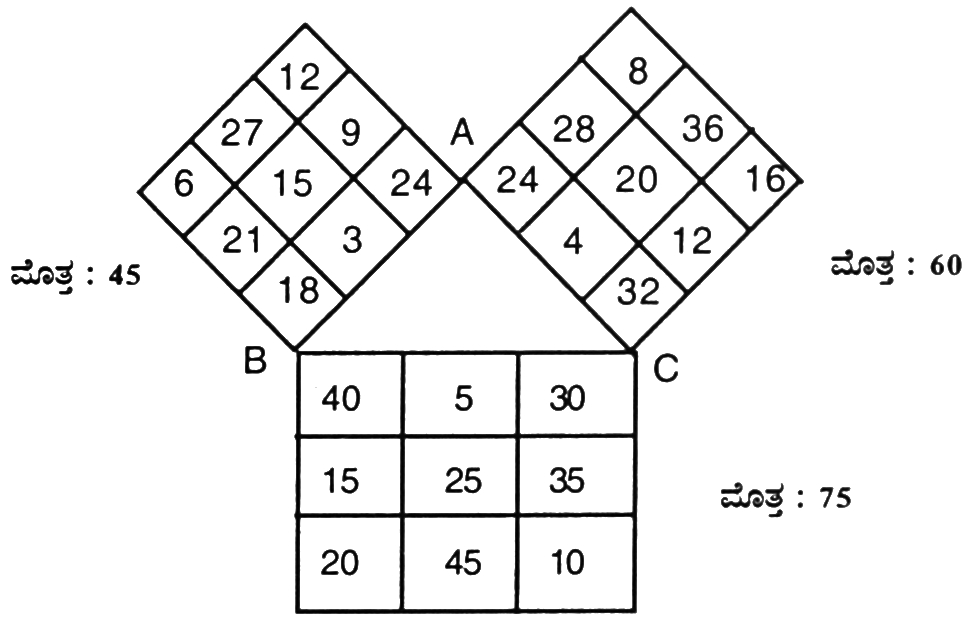
\includegraphics[scale=1.2]{src/figures/chap8/fig8-10.jpg}
\end{figure}
\begin{itemize}
	\item ಪ್ರತಿ ಬಾಹುವಿನ ಮೇಲಿರುವ 3 ಕ್ರಮವರ್ಗದ ಮಾಯಾಚೌಕಗಳಲ್ಲಿನ ಅನುರೂಪ ಮನೆಗಳಲ್ಲಿರುವ ಸಂಖ್ಯೆಗಳು ಪೈಥಾಗೊರಾಸ್ ತ್ರಿವಳಿಗಳು.

	ಉದಾ: $40^2 = 24^2 +32^2 ; 25^2 =15^2 +20^2 ; 20^2 =16^2+12^2$\smallskip
	\item ಮಾಯಾ ಚೌಕಗಳ ಮೊತ್ತಗಳೂ ಪೈಥಾಗೊರಾಸ್ ತ್ರಿವಳಿಗಳೇ 752 =452 +602
\end{itemize}
\eject

\section*{IX- 4. ಮಾಯಾ ಘನ (Magic Cube)}

ಪುಟ 83ರಲ್ಲಿನ 8 ಕ್ರಮವರ್ಗದ ಮಾಯಾಚೌಕವನ್ನು \textbf{‘‘ಮಾಯಾಘನ’’} ವೂ ಎಂದು ಹೇಳಿದೆವಲ್ಲವೆ. ಅದನ್ನು ಇಲ್ಲಿ ವಿನ್ಯಾಸಗೊಳಿಸಲಾಗಿದೆ.

ಮಾಯಾಚೌಕವನ್ನು 4 ಸಮಭಾಗಗಳಾಗಿ ಮಾಡಿದೆ. ಎಡ ಮೇಲ್ತುದಿಯ $4 \times 4$ ಚೌಕ\-ವನ್ನು ಒಂದು ಘನದ ಮೇಲಿನ ಮುಖದಲ್ಲಿ ಹೊಂದಿಸಿದೆ. ಉಳಿದ ಮೂರು $4 \times 4$ ಚೌಕ\-ಗಳನ್ನು ಪ್ರದಕ್ಷಿಣ ಕ್ರಮವಾಗಿ ತೆಗೆದುಕೊಂಡು ಘನದ ಮಧ್ಯಭಾಗದಿಂದ ತಳಭಾಗದವರೆಗೆ ಜೋಡಿಸಿದೆ. ಒಂದರ ಕೆಳಗೆ ಒಂದು ಬರುವಂತೆ.

ಈ ಆಕೃತಿಯಲ್ಲಿ ಪ್ರತಿ $4 \times 4$ಚೌಕದ ಅಡ್ಡಸಾಲು, ಕಂಭಸಾಲು ಮತ್ತು ಕರ್ಣಗಳ ಸಂಖ್ಯೆಗಳ ಮೊತ್ತ 130. ಹಾಗೆಯೇ ಮೇಲಿನಿಂದ ಕೆಳಕ್ಕೆ 4 ಅನುರೂಪ ಮನೆಗಳ ಸಂಖ್ಯೆತೆಗೆದು\-ಕೊಂಡರೂ ಮೊತ್ತ 130.

\begin{minipage}{4cm}
\begin{figure}[H]
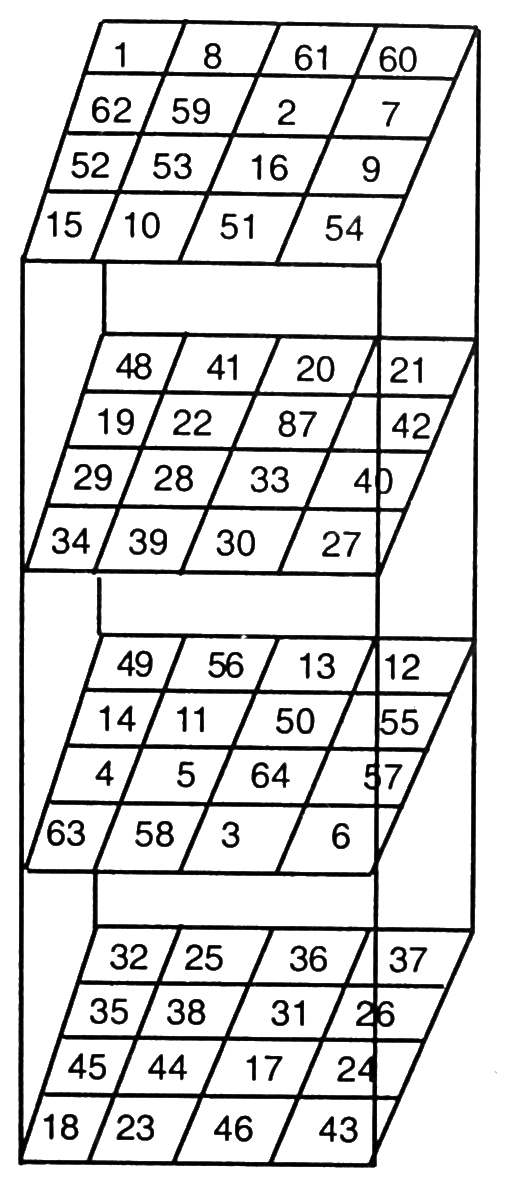
\includegraphics{src/figures/chap8/fig8-11.jpg}
\end{figure}
\end{minipage}
\quad
\begin{minipage}{5.5cm}
ಉದಾ : 15+34+63+18=130 53+28+5+44=130

ಮೇಲಿನ ಚೌಕದ ಯಾವುದೇ ಮೂಲೆಯ ಮನೆಯಿಂದ ಪ್ರಾರಂಭಿಸಿ ಅತಿ ಕೆಳಗಿನ ಎದುರು ಮೂಲೆಯ ಮನೆಗೆ ಎಳೆದ ಕರ್ಣದಲ್ಲಿ ಬರುವ ಸಂಖ್ಯೆಗಳ ಮೊತ್ತವೂ 130.

ಉದಾ : 1+22+64+43=130

ಉಳಿದ ಕರ್ಣಗಳ ಸಂಖ್ಯೆಗಳ ಮೊತ್ತವೂ 130.
\end{minipage}

\section*{IX- 5. ಜಾನಪದ ಒಗಟಿಗೆ ಮಾಯಾಚೌಕ ಪರಿಹಾರ :}

ಜಾನಪದ ಸಾಹಿತ್ಯದಲ್ಲಿ ಸಮಸ್ಯೆಗಳು/ಒಗಟುಗಳು ವಿಪುಲ. ಇವು ಸಾಮಾನ್ಯವಾಗಿ ಪದ್ಯರೂಪ\-ದಲ್ಲಿರುತ್ತವೆ. ಇಂತಹವುಗಳನ್ನು ಬಿಡುವಿನ ವೇಳೆಯ ಕಾಲಕ್ಷೇಪಕ್ಕೆ ಬಳಸುತ್ತಿದ್ದುದು ಈಗ್ಗೆ 60-70 ವರ್ಷಗಳ ಹಿಂದೆ ಕಾಣಸಿಗುತ್ತಿತ್ತು. ಇಂತಹ ಒಂದು ಸಮಸ್ಯೆಯನ್ನು ನೋಡೋಣ.

\medskip
\noindent \textbf{ಒಗಟು :} 
\begin{quote}
ಒಂಭತ್ತು ರಂಭೆಯರಿಗವನೊಬ್ಬ ಗಂಡ\\
ಎಂಭತ್ತೊಂದು ಎಮ್ಮೆಗಳ ತಾ ಕೊಂಡು ತಂದ\\
ಕುಂಭ ಕುಂಭಕೆ ಹೆಚ್ಚು ಹಾಲು ಕರಕೊಂಡ\\
ರಂಭೆಯರಿಗೆ ಇದ ಸಮ ಮಾಡಿಕೊಳ್ಳಿರೆಂದ
\end{quote}
(ಒಬ್ಬ ಕವಾಡಿಗ. ಅವನಿಗೆ 9 ಹೆಂಡತಿಯರು. ಅವನು 81 ಎಮ್ಮೆಗಳನ್ನು ಕೊಂಡು ತರುತ್ತಾನೆ. ಅವುಗಳು 1 ನೇ ಎಮ್ಮೆ 1 ಅಳತೆ ಹಾಲುಕೊಟ್ಟರೆ, 2ನೆಯದು 2 ಅಳತೆ, 3ನೆಯದು 3ಅಳತೆ, 4ನೆಯದು 4 ಅಳತೆ.........81ನೆಯದು 81 ಅಳತೆ ಹಾಲು ಕೊಡುತ್ತವೆ. ಎಮ್ಮೆಗಳ ಸಂಖ್ಯೆ, ಹಾಲಿನ ಪರಿಮಾಣ ಸಮವಾಗಿ ಬರುವಂತೆ 9 ಹೆಂಡತಿಯರಿಗೆ ಹಂಚಿ)

\medskip
\noindent \textbf{ಪರಿಹಾರ :}
\begin{itemize}
	\item ಒಟ್ಟು ಎಮ್ಮೆಗಳು 81; 9 ಜನರಿಗೆ ಸಮನಾಗಿ ಹಂಚಿದರೆ ಪ್ರತಿಯೊಬ್ಬರಿಗೂ 9 ಎಮ್ಮೆ ಬರುತ್ತದೆ.
	\item ಎಮ್ಮೆಗಳು ಕೊಡುವ ಹಾಲಿನ ಪರಿಮಾಣ 1+2+3+4.......+81 ಅಳತೆಗಳು \break ಅಂದರೆ $81 \times 82\div 2 = 3321$ ಅಳತೆಗಳು 9 ಜನರಿಗೆ ಸಮನಾಗಿ ಹಂಚಿದರೆ ಒಬ್ಬರಿಗೆ ಬರುವ ಹಾಲಿನ ಪರಿಮಾಣ $3321 \div 9 = 369$ ಅಳತೆಗಳು
\end{itemize}

\medskip
\noindent \textbf{ಪರಿಹಾರ :}
\begin{itemize}
	\item 1ರಿಂದ 81 ರವರೆಗಿನ ಸಂಖ್ಯೆಗಳನ್ನು ಬಳಸಿ 9 ಕ್ರಮವರ್ಗದ ಮಾಯಾಚೌಕ ರಚಿಸಿ.
	\item ಎಮ್ಮೆಗಳನ್ನು 1,2,3.....81ಎಂದು ಗುರ್ತಿಸಿದರೆ ಪ್ರತಿ ಹೆಂಡತಿಗೂ ಅಡ್ಡಸಾಲಿನ / ಕಂಭಸಾಲಿನ ಸಂಖ್ಯೆಗಳ 9 ಎಮ್ಮೆ ಹಂಚಬಹುದು.
	\item ಆಗ ಆ 9 ಎಮ್ಮೆಗಳು ಕೊಡುವ ಹಾಲಿನ ಪರಿಮಾಣವೂ ಸಮ. ಪ್ರತಿಯೊಂದೂ 369 ಅಳತೆಗಳು.
\end{itemize}
ಈ ಒಗಟಿಗೆ ಬೇರೆ ಬೇರೆ ರೀತಿಯ ಮಾಯಾಚೌಕಗಳನ್ನು ರಚಿಸಿ ಪರಿಹಾರ ನೀಡಬಹುದು. ಪ್ರಯತ್ನಿಸಿ.
\begin{figure}[H]
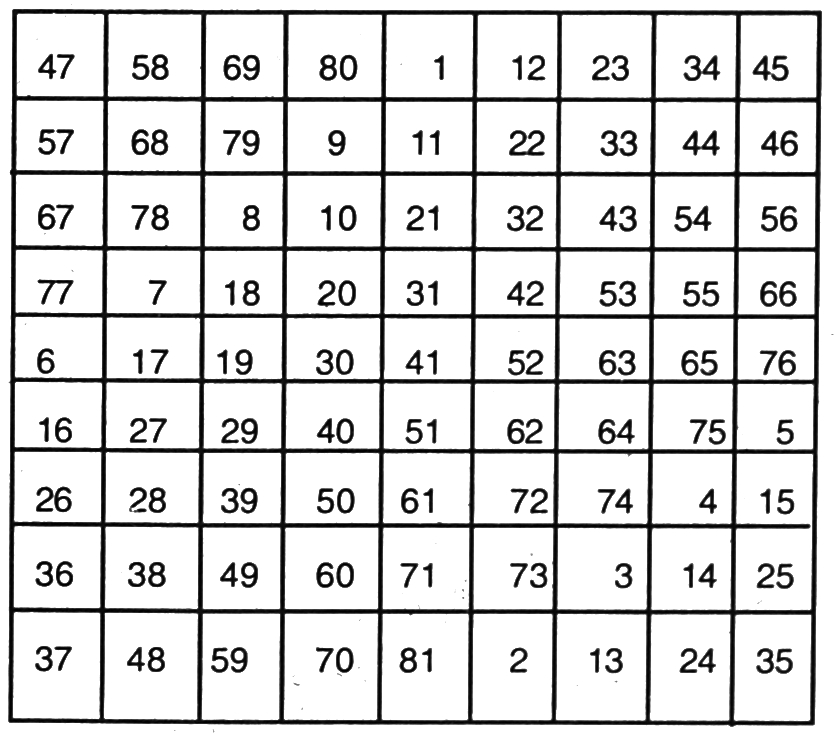
\includegraphics[scale=.85]{src/figures/chap8/fig8-12.jpg}
\end{figure}

\section*{IX- 6. ಮೈಸೂರು ಸಂಸ್ಥಾನದ ಮಹಾರಾಜರಾಗಿದ್ದ ಮುಮ್ಮಡಿ ಕೃಷ್ಣರಾಜ ಒಡೆಯರ್ (ಕ್ರಿ.ಶ. 1794-1868) ವಿರಚಿತ ‘‘ಚತುರಂಗ ಸಾರ ಸರ್ವಸ್ವ’’ ಕೃತಿಯಿಂದ,}

1 ರಿಂದ 88 ರ ವರೆಗೆ ಸಂಖ್ಯೆಗಳು ಕುದುರೆ ನಡಿಗೆಯಲ್ಲಿವೆ.
\begin{figure}[H]
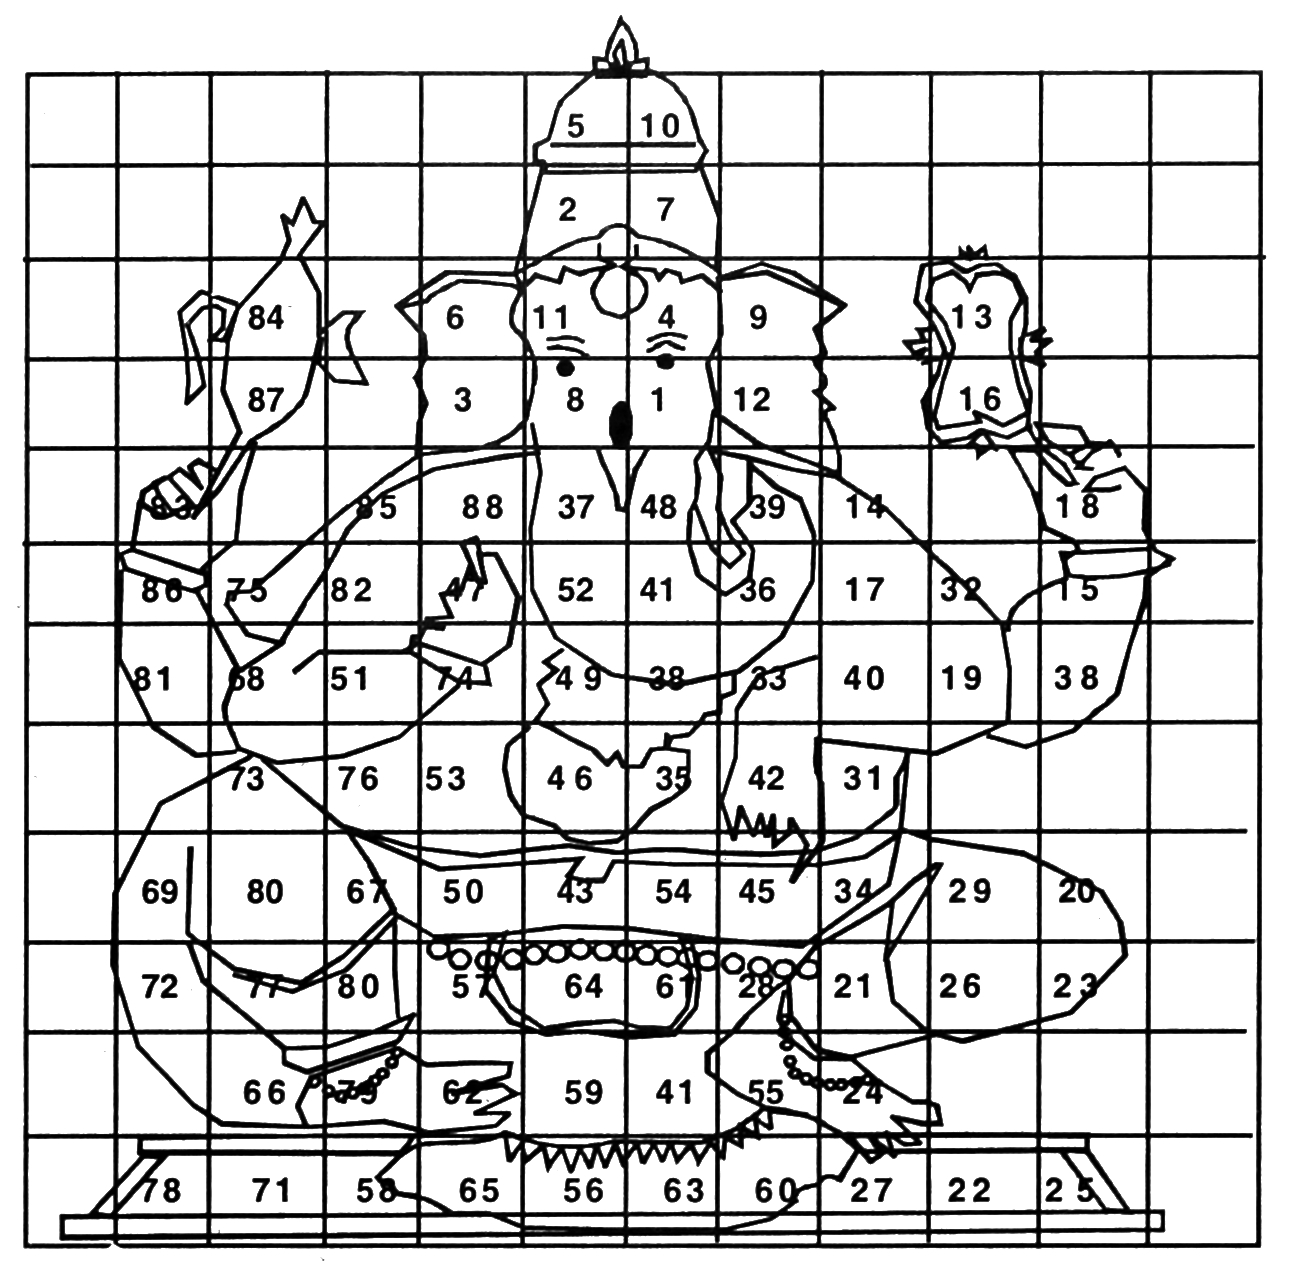
\includegraphics[scale=.75]{src/figures/chap8/fig8-13.jpg}
\end{figure}
